\chapter{Protocolos de Comunicación Serial}
\label{C:anexo-comunicación-serial}

\section{UART}

UART (Universal Asynchronous Receiver-Transmitter) \cite{fernandez-com-serial} es un protocolo de comunicación serial asincrónica y bidireccional full-duplex desarrollado en el año 1960 por la empresa Digital Equipment Corporation. Esta interfaz posee dos líneas de datos, RX y TX, las cuales se interconectan como lo muestra la figura~\ref{F:uart-interconexión}. UART generalmente es usada para establecer una comunicación bidireccional full-dúplex sólo entre dos dispositivos (punto a punto).

\begin{figure}[ht!]
\centering
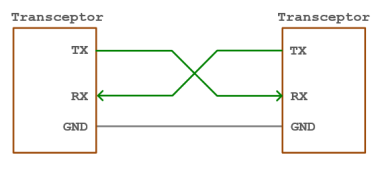
\includegraphics[width=0.55\textwidth]{./imagenes/uart-interconexión.png}
\caption{Interconexión de interfaz UART}
\label{F:uart-interconexión}
\end{figure}

La información intercambiada entre los dispositivos es mediante paquetes de datos con un formato definido como se muestra en la figura~\ref{F:uart-trama-datos}. La comunicación está sincronizada mediante los bits de START y STOP que posee el paquete, considerando que los relojes de los dispositivos transmisor y receptor operan a la misma frecuencia.

\begin{figure}[ht!]
\centering
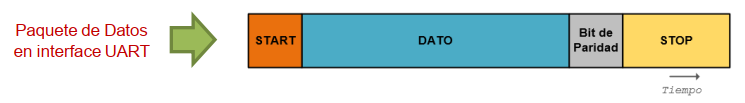
\includegraphics[width=0.9\textwidth]{./imagenes/uart-trama-datos.png}
\caption{Paquete de datos UART}
\label{F:uart-trama-datos}
\end{figure}

El paquete de datos indicado posee las siguientes configuraciones que deben efectuarse en los dispositivos que intervienen en la comunicación:

\begin{description}
   \item[Bit de START] Es el primer bit del paquete de datos y permite que el receptor reconozca el inicio de la transmisión de un paquete. Normalmente el transmisor (TX) mantiene la línea de datos en “1” cuando se encuentra en reposo. Para iniciar la transmisión pone a “0” la línea y el receptor, al detectar esto, comienza con la lectura del DATO.
   \item[DATO] Este campo del paquete puede configurarse de 5 a 9 bits. La configuración debe ser la misma para ambos dispositivos en la comunicación. Los bits son enviados uno a uno, empezando por el menos significativo y terminando con el más significativo.
   \item[Bit de Paridad] Permite al receptor verificar si los datos recibidos son correctos o no. La paridad es un sistema de comprobación de errores de bajo nivel y puede ser de paridad par o paridad impar. Debe configurarse la misma paridad en ambos dispositivos involucrados en la comunicación.
   \item[Bit de STOP] Marca el final del paquete de datos al receptor. Puede tener uno o dos bits de longitud. Debe configurarse lo mismo en ambos dispositivos. Al finalizar la transmisión, es habitual que se mantenga la línea de datos en “1” (línea en reposo).
   \item[Baud Rate (bits por segundo)]  Es un parámetro que indica la velocidad a la que se transmiten los datos y se relaciona con el reloj interno que poseen los dispositivos para la lectura/escritura de los bits que conforman el paquete de datos. Todos los dispositivos deben tener el mismo baud rate. Algunas de las velocidades estándares son 4800 bps, 9600 bps, 19200 bps, 115200 bps, etc. De estas, 9600 bps es la más utilizada.
\end{description}

\section{I\texorpdfstring{\textsuperscript{2}}{Lg}C}

I\textsuperscript{2}C (Inter-Integrated Circuit) \cite{fernandez-com-serial} es un bus de comunicación serie sincrónica bidireccional half-duplex desarrollado en el año 1982 por la empresa Philips Semiconductors. El bus I2C también es conocido con el nombre de TWI (Two Wire Interface). Este bus también posee una arquitectura Maestro-Esclavo, donde el dispositivo Maestro es el único que puede iniciar y finalizar la transmisión y también proveer la señal de reloj. En I2C los dispositivos Esclavos pueden convertirse en Maestros, pero en el bus sólo puede existir un Maestro a la vez.

El bus está compuesto de dos líneas y la conexión común de GND, como puede apreciarse en la figura~\ref{F:i2c-interconexión}. Existe una línea bidireccional para el intercambio de datos que se denomina SDA (Serial Data) y una para la señal de reloj denominada SCL (Serial Clock). Como en este bus no existen líneas de selección de esclavo, cada dispositivo Esclavo debe contar con una dirección única (código de identificación) la cual debe incluirse al dato. Esto resulta en una reducción de la velocidad de transferencia de cada byte de dato.

Las líneas SDA y SCL son del tipo drenador abierto (figura~\ref{F:i2c-entrada-y-salida}), por lo cual cada una requiere una resistencia pull-up Rp ($ \num{1.8}~\unit{\kilo\Omega} \leq Rp \leq \num{10}~\unit{\kilo\Omega} $).

\begin{figure}[ht!]
\centering
\subfloat[Interconexión de interfaz I\textsuperscript{2}C][Interconexión de interfaz I\textsuperscript{2}C]{
	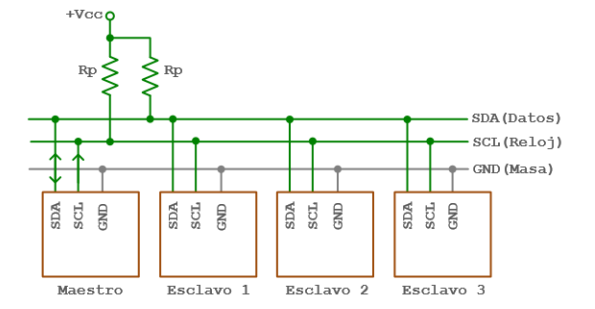
\includegraphics[width=0.65\textwidth]{./imagenes/i2c-interconexión.png}
	\label{F:i2c-interconexión}}
\\
\subfloat[Líneas SDA y SCL][Líneas SDA y SCL]{
	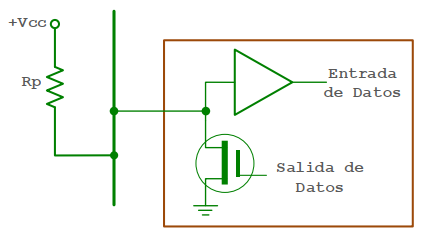
\includegraphics[width=0.43\textwidth]{./imagenes/i2c-entrada-y-salida.png}
	\label{F:i2c-entrada-y-salida}}
\caption{Interfaz I\textsuperscript{2}C}
\end{figure}

A continuación se describe un ejemplo de trama del protocolo I\textsuperscript{2}C, la cual se puede observar en la figura~\ref{F:i2c-trama-y-sec}:

\begin{itemize}
    \item El Maestro inicia la comunicación con la secuencia de inicio (START), acompañada de 7~bits que corresponden a la dirección del Esclavo con el que se desea comunicar. A esto el Maestro agrega un bit que indica si la operación será de escritura (W~=~0) o  de lectura (R~=~1). En este caso de escritura.
    \item Si el Esclavo está disponible en el bus, responde con un bit de reconocimiento (ACK) a lo anterior. Si no hay respuesta del Esclavo en cuestión, el Maestro terminará la comunicación con una secuencia de parada (STOP).
    \item Luego de que el Maestro recibe el bit de reconocimiento, el mismo envía el Dato~1 (de 8~bits) que corresponde a la dirección del registro del Esclavo donde se desea escribir. A esto el Esclavo vuelve a responder con un bit de reconocimiento (ACK). Si esto no sucede el Maestro finaliza la comunicación con una secuencia de parada (STOP).
    \item Recibido el bit de reconocimiento, el Maestro envía el Dato~2 (8~bits) que corresponde al valor que se cargará en el registro del Esclavo. Luego, este último responde con un bit de reconocimiento (ACK). Caso contrario, el Maestro finaliza la comunicación.
    \item Una vez que el Maestro ha escrito el valor correspondiente (Dato~2) en el registro deseado (Dato~1) del Esclavo, finaliza la comunicación con una secuencia de parada (STOP).
\end{itemize}

\begin{figure}[ht!]
\centering
\subfloat[Ejemplo de trama I\textsuperscript{2}C: Escritura en el registro de un Esclavo (M: Maestro; E: Esclavo)][Ejemplo de trama I\textsuperscript{2}C: Escritura en el registro de un Esclavo (M: Maestro; E: Esclavo)]{
	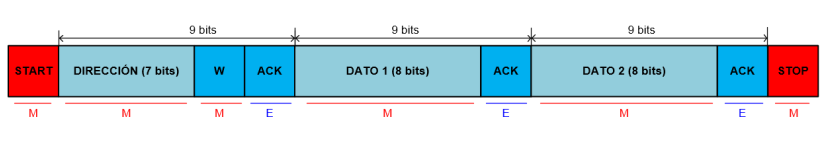
\includegraphics[width=0.98\textwidth]{./imagenes/i2c-trama.png}
	\label{F:i2c-trama}}
\\
\subfloat[Secuencia de inicio y parada I\textsuperscript{2}C][Secuencia de inicio y parada I\textsuperscript{2}C]{
	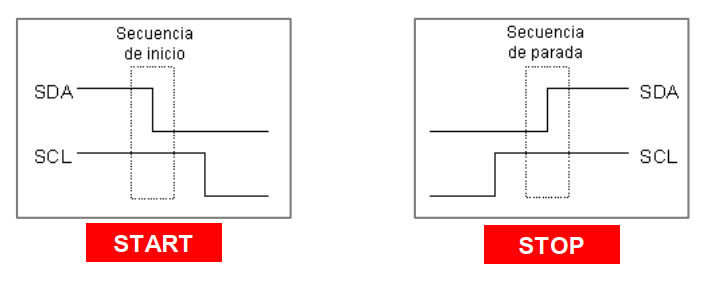
\includegraphics[width=0.7\textwidth]{./imagenes/i2c-sec-inicio-parada.png}
	\label{F:i2c-sec-inicio-parada}}
\caption{Trama y secuencia de inicio y parada I\textsuperscript{2}C}
\label{F:i2c-trama-y-sec}
\end{figure}

En la figura~\ref{F:i2c-trama-en-detalle} se encuentra ilustrada en forma más detallada la trama I\textsuperscript{2}C. A continuación se describen cada una de las subfiguras.

\paragraph{Reconocimiento de bits (figura~\ref{F:i2c-fig1}):}
El nivel lógico de la línea SDA debe ser estable cuando la línea SCL es alta. La única excepción a esta regla es la generación de secuencias de START y STOP.

\paragraph{Secuencias de START y STOP (figura~\ref{F:i2c-fig2}):}
El bus está inactivo cuando SDA~=~1 y SCL~=~1. El Maestro inicia la transmisión con una secuencia START (SDA~=$ \downarrow $  con SCL~=~1) y finaliza la misma con una secuencia de STOP (SDA~=~$ \uparrow $ con SCL~=~1). Entre una condición de START y STOP, el bus se considera ocupado y ningún otro maestro debe intentar tomar el control del bus. Si el Maestro genera una nueva secuencia de START antes de la secuencia de STOP, esto se conoce como INICIO REPETIDO (\textit{Repeated START}) y se utiliza cuando el Maestro desea iniciar una nueva transferencia sin renunciar al control del bus.

\paragraph{Paquete de Dirección (figura~\ref{F:i2c-fig3}):}
Todos los paquetes de direcciones transmitidos tienen una longitud de 9~bits y están constituidos
por:

\begin{itemize}
    \item 7~bits más significativos para la dirección del Esclavo con el cual el Maestro desea comunicarse.
    \item 1~bit para definir la operación que desea realizar el Maestro. Puede ser Lectura (R) o Escritura ($ \overline{\text{W}} $). Este bit debe ser “1” para el caso de lectura y “0” para escritura.
    \item 1~bit de reconocimiento (ACK). Este bit es generado por el Esclavo cuando reconoce la dirección enviada por el Maestro. El esclavo debe poner a “0” la línea SDA si reconoce la dirección.
\end{itemize}

\paragraph{Paquete de Datos (figura~\ref{F:i2c-fig4}):}
Todos los paquetes de datos transmitidos poseen una longitud de 9~bits y están constituidos por:

\begin{itemize}
    \item 8~bits para datos.
    \item 1~bit de reconocimiento (ACK). Este bit es generado por el receptor de los datos. El reconocimiento de la recepción se efectúa poniendo en “0” la línea SDA durante el noveno ciclo de reloj en línea SCL. Si el receptor deja la línea SDA en “1”, se señaliza un NACK. Esta señalización permite al receptor avisar que ha recibido el último byte, o por alguna razón no puede recibir más bytes.
\end{itemize}

\paragraph{Combinación de Paquetes de Dirección y Datos (figura~\ref{F:i2c-fig5}):}
 Una transmisión consiste básicamente en una secuencia de START, una dirección más bit R o W (SLA+R/W)\footnote{SLA significa dirección de esclavo (Slave Address)}, uno o más paquetes de datos y una secuencia de STOP. Pueden existir varios bytes de datos entre SLA+R/W y STOP, dependiendo del protocolo implementado por el programa del usuario.

\vspace{4cm}
~

\begin{figure}[H]
\centering
\subfloat[Reconocimiento de bits][Reconocimiento de bits]{
	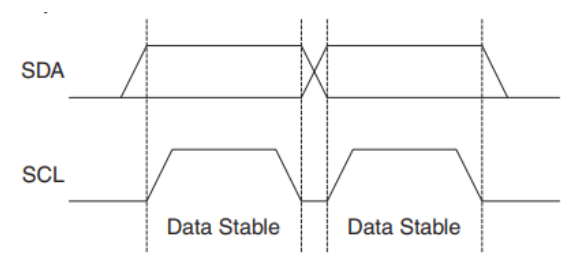
\includegraphics[width=0.41\textwidth]{./imagenes/i2c-fig1.png}
	\label{F:i2c-fig1}}
\quad
\subfloat[Secuencias de START y STOP][Secuencias de START y STOP]{
	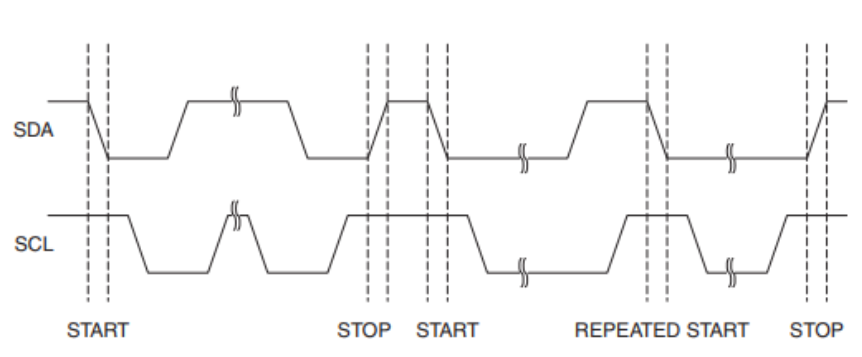
\includegraphics[width=0.53\textwidth]{./imagenes/i2c-fig2.png}
	\label{F:i2c-fig2}}
\\
\subfloat[Paquete de Dirección][Paquete de Dirección]{
	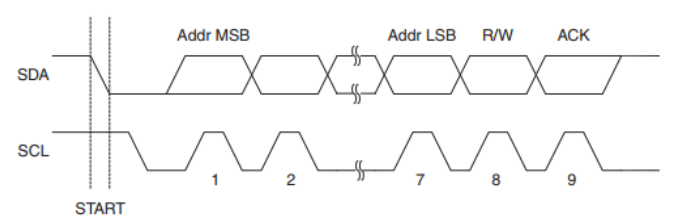
\includegraphics[width=0.62\textwidth]{./imagenes/i2c-fig3.png}
	\label{F:i2c-fig3}}
	\\
\subfloat[Paquete de Datos][Paquete de Datos]{
	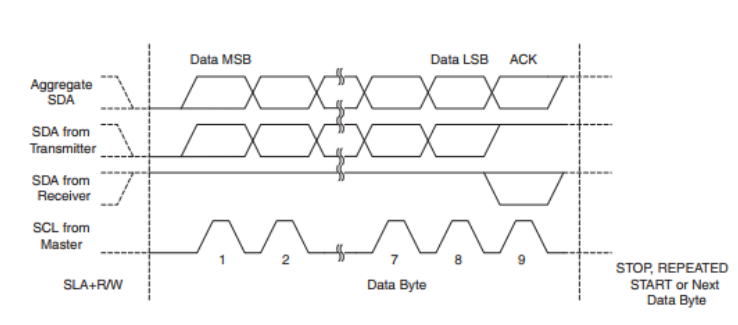
\includegraphics[width=0.75\textwidth]{./imagenes/i2c-fig4.png}
	\label{F:i2c-fig4}}
	\\
\subfloat[Combinación de Paquetes de Dirección y Datos][Combinación de Paquetes de Dirección y Datos]{
	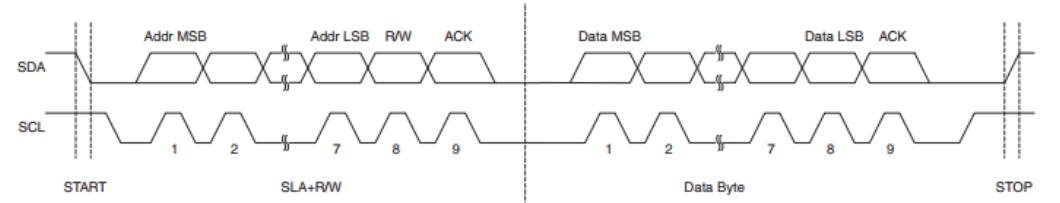
\includegraphics[width=0.95\textwidth]{./imagenes/i2c-fig5.png}
	\label{F:i2c-fig5}}
\caption{Trama I\textsuperscript{2}C en detalle}
\label{F:i2c-trama-en-detalle}
\end{figure}

\section{SPI}

SPI (Serial Peripheral Interface) \cite{fernandez-com-serial} es un bus de comunicación serie sincrónica bidireccional full-duplex desarrollado en el año 1980 por la empresa Motorola. En el bus SPI hay un dispositivo Maestro y uno o más Esclavos. El Maestro es el único encargado de iniciar y finalizar la comunicación en cualquiera de las direcciones y también genera la señal de reloj de sincronización. Este bus se encuentra compuesto por las siguientes cuatro líneas más la línea común de GND:
\clearpage
\begin{description}
   \item[MOSI (Master Out Slave In):] Esta línea lleva los datos desde el Maestro a los Esclavos.
   \item[MISO (Master In Slave Out):] Lleva los datos desde los Esclavos al Maestro.
   \item[CLK (Clock):] Esta línea lleva los pulsos de reloj desde el Maestro a los Esclavos.
   \item[$ \overline{\text{SS}} $ (Slave Select):] Es la línea mediante la cual el Maestro selecciona al Esclavo con el cual quiere comunicarse. Si hay varios esclavos, pueden existir varias líneas de selección de esclavos.
\end{description}

\begin{figure}[ht!]
\centering
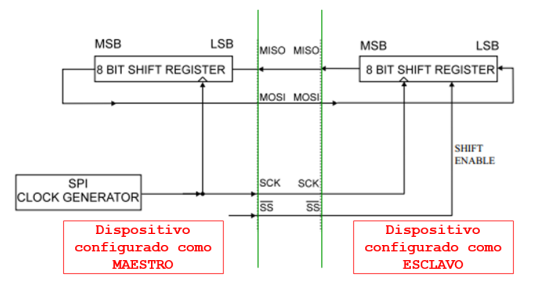
\includegraphics[width=0.8\textwidth]{./imagenes/spi-interconexión.png}
\caption{Interconexión interfaz SPI}
\label{F:spi-interconexión}
\end{figure}


\paragraph{Operación:}
El sistema de comunicación SPI de la figura~\ref{F:spi-interconexión} posee dos registros de desplazamiento (de 8 bits c/u) y un generador de reloj maestro. El maestro SPI inicia el ciclo de comunicación cuando pone en bajo el pin $ \overline{\text{SS}} $. El maestro y el esclavo preparan los datos para ser enviados en sus respectivos registros de desplazamiento, y el maestro genera los pulsos de reloj requeridos en la línea CLK para intercambiar los datos. Estos últimos van de Maestro a Esclavo a través de la línea MOSI y de Esclavo a Maestro a través de MISO. Después de cada paquete de datos (8 bits), el maestro sincronizará al esclavo poniendo en alto la línea de selección $ \overline{\text{SS}} $.